
% utf-8
\documentclass[notes=hide]{beamer}
\usepackage[utf8]{inputenc}
\usepackage[ngerman,english]{babel}
 \usepackage{ngerman}
\usepackage{graphicx}
\usepackage{wasysym}
\usepackage{alltt}
\usepackage{bbm}
\usepackage{stmaryrd}
\usepackage{eurosym}
\usepackage{bm}
\usepackage{xfrac}
\usepackage{hyperref}

\usetheme{uds}

\setbeamerfont{smallfont}{size=\small}
\setbeamerfont{smallerfont}{size=\footnotesize}
\setbeamerfont{smallestfont}{size=\scriptsize}
\setbeamerfont{tinyfont}{size=\tiny}
\setbeamerfont{largefont}{size=\large}
\setbeamerfont{Largefont}{size=\LARGE}

\newcommand\bluebox[2][uds@main]{{%
  \setlength{\fboxsep}{0pt}%
  \colorbox{#1}{#2\strut}%
}}

\def\Prob{\mbox{\bf P}}
\newcommand{\OO}{\mathcal{O}}
\newcommand{\N}{\mathbbm{N}}
\newcommand{\len}[1]{{\vert #1 \vert}}
\newcommand{\emptystring}{\varepsilon}
\newcommand{\substr}[3]{#1[#2\ldots#3]}
\newcommand{\suffix}[2]{{#1}[{#2}\ldots]}
\newcommand{\prefix}[2]{{#1}[\ldots{#2}]}
\newcommand{\chr}[2]{#1[#2]}
\newcommand{\powset}[1]{2^{#1}}
\newcommand{\pos}{\ensuremath{\texttt{\upshape pos}}}
\newcommand{\lcp}{\ensuremath{\texttt{\upshape lcp}}}
\newcommand{\cld}{\ensuremath{\texttt{\upshape cld}}}
\newcommand{\rank}{\ensuremath{\texttt{\upshape rank}}}
\newcommand{\bwt}{\ensuremath{\texttt{\upshape bwt}}}
\newcommand{\bwtfind}{\ensuremath{\texttt{\upshape bwtfind}}}
\newcommand{\Occ}{\ensuremath{\texttt{\upshape Occ}}}
\newcommand{\less}{\ensuremath{\texttt{\upshape less}}}
\newcommand{\type}{\ensuremath{\texttt{\upshape type}}}
\newcommand{\lcpskip}{\ensuremath{\texttt{\upshape skip}}}
\newcommand{\gap}{\ensuremath{\text{--}}}
\newcommand{\iverl}{\llbracket}
\newcommand{\iverr}{\rrbracket}
\newcommand{\C}{\ensuremath{\texttt{\upshape C}}}

\newcommand{\0}{\ensuremath{\mathtt{0}}}
\newcommand{\1}{\ensuremath{\mathtt{1}}}

\newcommand{\rz}{\red\0}
\newcommand{\ro}{\red\1}
\newcommand{\gz}{\green\0}
\newcommand{\go}{\green\1}
\newcommand{\bz}{\blue\0}
\newcommand{\bo}{\blue\1}

\newcommand{\at}{\atopwithdelims..}
\newcommand{\atb}{\atopwithdelims\{\}}
\newcommand{\snp}[2]{\{\blue{#1},\blue{#2}\}}

\newcommand{\mathds}[1]{#1}
\def\cA{\mathcal{A}}
\def\cC{\mathcal{C}}
\def\cN{\mathcal{N}}
\def\cS{\mathcal{S}}
\def\cR{\mathcal{R}}
\def\vG{\mathbf{G}}
\def\vP{\mathbf{P}}
\DeclareMathOperator*{\argmax}{arg\,max}

\newcommand{\blackboard}[1]{
\begin{block}<#1>{}
\begin{center}
\textbf{BLACK BOARD EXAMPLE}
\end{center}
\end{block}
}

\usepackage{listings} % ab Version 1.4 mit Python-Syntax-Highlighting!
\definecolor{mygray}{gray}{.50}
\lstset{language=Python,
    basicstyle=\small\ttfamily,
    stringstyle=\ttfamily\color{green},
    keywordstyle=\color{blue}\bfseries,
    commentstyle=\color{mygray},
    tabsize=4,
    numbers=left,
    numberstyle=\tiny,
    numbersep=5pt,
    morekeywords=assert,
    extendedchars=false,
    showstringspaces=false,
    frame=single
    }
\lstset{escapeinside={/*@}{@*/}}

\newcommand{\captionslide}[1]{
\begin{frame}
\frametitle{\phantom{NONE}}
\begin{center}
\vspace{1cm}
\usebeamerfont{Largefont}
          {\bf\em #1}
          \vspace{2cm}
\end{center}
\end{frame}
}


\title{Day 2: Brief HIV Primer}
\author[TM]{Jordan Eizenga, Erik Garrison and Tobias Marschall}
\date{CPANG18 @ Instituto Gulbenkian de Ci\^{e}ncia\\ March, 2018}

\begin{document}

\frame[plain]{\titlepage}

% \begin{frame}{Topics}
% \begin{block}{Past-/Current}
% \begin{itemize}
%  \item long-indel-aware read mapping
%  \item for calling and genotyping structural variations
%  \item for read-based phasing of diploid samples
%  \item for haplotype reconstruction and quantification of virus populations
%  \item for detecting motif-induced sequencing errors in Illumina data
%  \item for calling somatic mutations in cancer.
%  \item GoNL
% \end{itemize}
% \end{block}
% \begin{block}{Current-/Future}
% \begin{itemize}
%  \item Bacterial GWAS
%  \item HGT
% \end{itemize}
% \end{block}
% \end{frame}

\setbeamertemplate{footline}{\hfill\insertframenumber{}\hspace*{10pt}\vskip10pt}

\begin{frame}{Viral Quasispecies}
\textit{``Virologists use the term viral quasispecies to mean distributions of nonidentical but related genomes subjected to a continuous process of genetic variation, competition, and selection and which act as a unit of selection.''}\\
(Domingo, Sheldon and Perales, MMBR, 2012)
\end{frame}

\begin{frame}{Viral Quasispecies}
\begin{center}
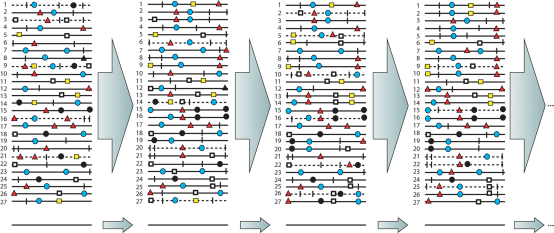
\includegraphics[width=\textwidth]{figs/quasispecies-model}\\[.5em]
{\scriptsize Figure from Domingo, Sheldon and Perales (2012)}
\end{center}
\begin{block}{}
\centering \emph{HIV forms quasispecies within hosts.} 
\end{block}
\end{frame}

\begin{frame}
\frametitle{Intra-Patient Viral Diversity}
\begin{center}
\includegraphics[width=\textwidth]{figs/intra-patient-diversity}
\end{center}
\end{frame}

\begin{frame}
\frametitle{Quasispecies Assembly Workflow}
\begin{center}
\includegraphics[width=\textwidth]{figs/workflow-overview}
\end{center}
\end{frame}


\begin{frame}
\frametitle{How HIV Enters a Cell}
\begin{center}
\includegraphics[width=\textwidth]{figs/hiv-cell-entry}\\
{\tiny Source: Wilen, Tilton, Doms, Cold Spring Harb Perspect Med., 2012.}
\end{center}
\end{frame}

\begin{frame}{Deep Sequence Reveals Diversity}
\begin{center}
\includegraphics[width=\textwidth]{figs/hiv-env-v3-sanger-vs-ngs}\\
{\tiny Source: Qui\~{n}ones-Mateu et al., J Clin Virol., 2015.}
\end{center}
\begin{block}{}
\centering \emph{Phylogeny of HIV-1 V3 region of gp120 (env gene)} 
\end{block}
\end{frame}

\begin{frame}{Alignment Artifacts Hamper Analysis}
 \begin{center}
\includegraphics[width=\textwidth]{figs/5-virus-env-loop-igv-gap-wander}\\
\end{center}
\begin{block}{}
\centering \emph{Gap wander in alignments to env loop regions} 
\end{block}
\end{frame}

\begin{frame}{Data Set for Today: Five Virus Lab Mix}
 \begin{center}
\includegraphics[width=\textwidth]{figs/5vm_workflow.png}\\
{\tiny https://github.com/cbg-ethz/5-virus-mix\\ Di Giallonardo, et al., NAR, 2014.}
\end{center}
% \begin{block}{}
% \centering \emph{Gap wander in alignments to env loop regions} 
% \end{block}
\end{frame}

\end{document}


